\subsubsection{UserController}
\begin{figure}[h]
\centering
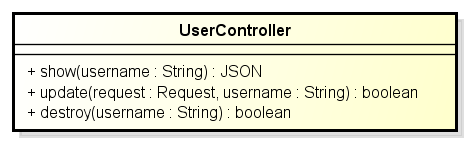
\includegraphics[width=0.5\linewidth]{img/back_end_http_controllers_userController}
\caption[Diagramma della classe UserController]{Diagramma della classe UserController}
\label{fig:back_end_http_controllers_userController}
\end{figure}

	\paragraph{Descrizione}
		Questa classe gestisce i dati dell'utente sfruttando i dati forniti dal model.
	\paragraph{Utilizzo}
		La classe è progettata per consentire la creazione, la manipolazione  dei dati utente e l'interrogazione efficiente del database.

	\paragraph{Metodi}
		\begin{itemize}
			\item \textbf{+ show(username = "")}\\
			Il metodo verifica se c'è un utente autenticato. Se la verifica ha avuto successo si procede con il recupero dei dati dell'utente, in particolare il suo profilo e i progetti associati all'utente e restituisce un oggetto JSON contenente le informazioni:\\
			\textbf{Argomenti}
			\begin{itemize}
				\item username : string = "";\\
				Stringa contenente il nome utente con valore di default NULL.
			\end{itemize}
			
			\item \textbf{+ update()}\\
			Il metodo recupera l'utente loggato e aggiorna i dati del profilo. Il metodo ritorno un valore boolean che indica se i dati sono stati aggiornati o meno;
			
			\item \textbf{+ destroy()}
			Il metodo recupera l'utente loggato e lo cancella dal database insieme a tutte le  sue informazioni. Il metodo ritorna un valore boolean che indica se è stato cancellato o meno dal database.
		\end{itemize}
		
\newpage
\subsubsection{ProjectController}
\begin{figure}[h]
\centering
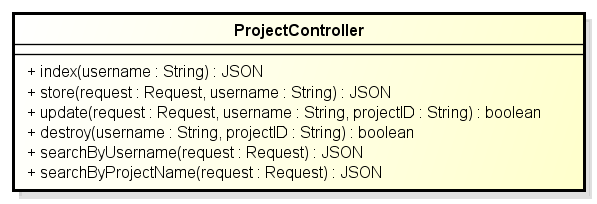
\includegraphics[width=0.5\linewidth]{img/back_end_http_controllers_projectController}
\caption[Diagramma della classe ProjectController]{Diagramma della classe ProjectController}
\label{fig:back_end_http_controllers_projectController}
\end{figure}

	\paragraph{Descrizione}
		Questa classe gestisce i dati di un progetto.
	\paragraph{Utilizzo}
		La classe è progettata per consentire la creazione e la manipolazione dei dati di un progetto.
		
	\paragraph{Metodi}
		\begin{itemize}
			\item \textbf{+ index()}\\
			Il metodo recupera tutti i progetti dell'utente loggato e li restituisce. Il metodo restituisce un JSON con le informazioni richieste;
			\item \textbf{+ store()}\\
			Il metodo crea un nuovo progetto assegnandoli un nome e lo salva nel database. Il metodo restituisce un valore boolean che indica se le informazioni sono state salvate o meno nel database;
			\item \textbf{+ show(project)}\\
			Il metodo interroga il database recuperando il progetto con l'id "project". Il metodo ritorna un JSON con le informazioni di un progetto:\\
			\textbf{Argomenti}
			\begin{itemize}
				\item project : string; \\
				Stringa contenente l'id univoco di un progetto.
			\end{itemize}
			\item \textbf{+ update(project)}\\
			Il metodo recupera il progetto e aggiorna i dati del progetto. Il metodo ritorna un valore boolean che indica se l'aggiornamento delle informazioni è avvenuto o meno:\\
			\textbf{Argomenti}
			\begin{itemize}
				\item project : string; \\
				Stringa contenente l'id univoco di un progetto.
			\end{itemize}
			\item \textbf{+ destroy(project)}\\
			Il metodo recupera il progetto e lo cancella dal database insieme a tutte le  sue informazioni. Il metodo ritorna un valore boolean che indica se la cancellazione del progetto dal database è avvenuta o meno:\\
			\textbf{Argomenti}
			\begin{itemize}
				\item project : string; \\
				Stringa contenente l'id univoco di un progetto.
			\end{itemize}
		\end{itemize}
		
\newpage
\subsubsection{InfographicController}
\begin{figure}[h]
\centering
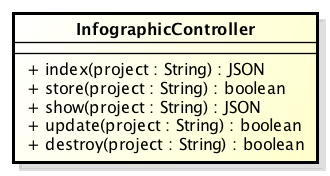
\includegraphics[width=0.5\linewidth]{img/back_end_http_controllers_infographicController}
\caption[Diagramma della classe InfographicController]{Diagramma della classe InfographicController}
\label{fig:back_end_http_controllers_infographicController}
\end{figure}

	\paragraph{Descrizione}
		Questa classe gestisce i dati di un'infografica.
	\paragraph{Utilizzo}
		La classe è progettata per consentire la creazione e la manipolazione dei dati di un infografica.
		
	\paragraph{Metodi}
		\begin{itemize}
			\item \textbf{+ index(project)}\\
			Il metodo recupera il progetti dell'utente loggato con id = project per poi ricavarsi l'infografica associato a tale progetto e restituisce un oggetto JSON con tutte le infografiche associate al progetto;
			\item \textbf{+ store(project)}\\
			Il metodo crea una nuova infografica assegnandoli un nome e il path per il salvataggio e la salva nel progetto con id = project. Il metodo ritorno un valore boolean che indica se il salvataggio è avvenuto o meno;
			\item \textbf{+ show(project, infographic)}\\
			Il metodo interroga il database recuperando il progetto con l'id "project" e a partire dal progetto recupera l'infografica con id = infographic. Il metodo ritorna un oggetto JSON con le informazioni richieste di una infografica:\\
			\textbf{Argomenti}
			\begin{itemize}
				\item project : string; \\
				Stringa contenente l'id univoco di un progetto;
				\item infographic : string; \\
				Stringa contenente l'id univoco di un'infografica.
			\end{itemize}
			\item \textbf{+ update(project, infographic)}\\
			Il metodo recupera il progetto con id = project e a partire dal progetto recupera l'infografica con id = infografica e aggiorna i dati dell'infografica. Il metodo ritorna un valore boolean che indica se l'aggiornamento è stato effettuato o meno:\\
			\textbf{Argomenti}
			\begin{itemize}
				\item project : string; \\
				Stringa contenente l'id univoco di un progetto;
				\item infographic : string; \\
				Stringa contenente l'id univoco di un'infografica.
			\end{itemize}
			\item \textbf{+ destroy(project, infographic)}\\
			Il metodo recupera il progetto con id = project e a partire dal progetto recupera l'infografica con id = infografica chiamando il metodo delete su tale infografica cancellandola dal database. Il metodo ritorna un valore boolean che indica se la cancellazione è avvenuta o meno:\\
			\textbf{Argomenti}
			\begin{itemize}
				\item project : string; \\
				Stringa contenente l'id univoco di un progetto;
				\item infographic : string; \\
				Stringa contenente l'id univoco di un'infografica.
			\end{itemize}
		\end{itemize}
		
\newpage
\subsubsection{PresentationController}
\begin{figure}[h]
\centering
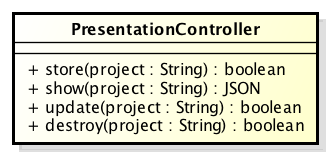
\includegraphics[width=0.5\linewidth]{img/back_end_premi_http_controllers_presentationController}
\caption[Diagramma della classe PresentationController]{Diagramma della classe PresentationController}
\end{figure}


	\paragraph{Descrizione}
		Questa classe gestisce i dati della presentazione.
	\paragraph{Utilizzo}
		La classe è stata progettata per consentire la creazione e la manipolazione dei dati di una presentazione.
	
	\paragraph{Metodi}
		\begin{itemize}
			\item \textbf{+ store(project)}\\
			Il metodo crea una nuova presentazione associata al progetto con id = project, assegnandole un titolo e la salva nel database: Il metodo ritorna un valore boolean che indica se il salvataggio nel database è avvenuto o meno:\\
			\textbf{Argomenti}
			\begin{itemize}
				\item project : string; \\
				Stringa contenente l'id univoco di un progetto.
			\end{itemize}
			\item \textbf{+ show(project)}\\
			Il metodo interroga il database recuperando il progetto con l'id "project" e restituisce l'unica presentazione associata a tale progetto. Il metodo ritorna un oggetto JSON contenente le informazioni di una presentazione:\\
			\textbf{Argomenti}
			\begin{itemize}
				\item project : string; \\
				Stringa contenente l'id univoco di un progetto.
			\end{itemize}
			\item \textbf{+ update(project)}\\
			Il metodo recupera il progetto con id = project per poi recuperare l'unica presentazione associata a tale progetto e aggiorna i dati della presentazione. Il metodo ritorna un valore boolean che indica se l'aggiornamento è stato effettuato o meno:\\
			\textbf{Argomenti}
			\begin{itemize}
				\item project : string; \\
				Stringa contenente l'id univoco di un progetto.
			\end{itemize}
			\item \textbf{+ destroy(project)}\\
			Il metodo recupera il progetto con id = project e recupare la presentazione associata a tale progetto e la elimina dal database cancellando tutte le sue informazioni. Il metodo ritorna un valore boolean che indica se la cancellazione nel database è avvenuta o meno:\\
			\textbf{Argomenti}
			\begin{itemize}
				\item project : string; \\
				Stringa contenente l'id univoco di un progetto.
			\end{itemize}
		\end{itemize}
		
\newpage
\subsubsection{SlideController}
\begin{figure}[h]
\centering
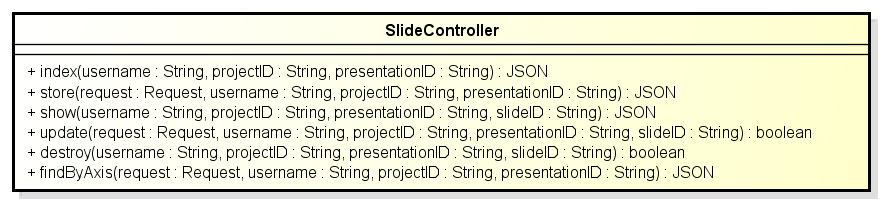
\includegraphics[width=0.5\linewidth]{img/back_end_http_controllers_slideController}
\caption[Diagramma della classe SlideController]{Diagramma della classe SlideController}
\label{fig:back_end_http_controllers_slideController}
\end{figure}

	\paragraph{Descrizione}
		Questa classe gestisce i dati di una slide.
	\paragraph{Utilizzo}
		La classe è stata progettata per consentire la creazione e la manipolazione dei dati di una slide.

	\paragraph{Metodi}
		\begin{itemize}
			\item \textbf{+ index(project)}\\
				Il metodo recupera e restituisce tutte le slide associate a una presentazione. Il metodo ritorna un oggetto JSON contenente le slide all'interno della presentazione:\\
				\textbf{Argomenti:}
				\begin{itemize}
					\item project : string; \\
					Stringa contenente l'id univoco di un progetto;
				\end{itemize}
			\item \textbf{+ store(project)}\\
				Il metodo crea una nuova slide.Il metodo ritorna un valore boolean che indica se l'aggiornamento è stato effettuato o meno:\\
				\textbf{Argomenti:}
				\begin{itemize}
					\item project : string; \\
					Stringa contenente l'id univoco di un progetto;
				\end{itemize}
			\item \textbf{+ show(project, slide)}\\
				Il metodo interroga il database recuperando la slide con id = slide. Il metodo ritorna un oggetto JSON contenente tutte le slide associate al progetto:\\
				\textbf{Argomenti:}
					\begin{itemize}
						\item project : string; \\
						Stringa contenente l'id univoco di un progetto;
						\item slide : string;\\
						Stringa contenente l'id univoco di una slide.
					\end{itemize}
			\item \textbf{+ update(project, slide)}\\
				Il metodo recupera il progetto con id = project per poi recuperare l'unica presentazione associata a tale progetto e la slide con id = slide aggiornando i dati della slide. Il metodo ritorna un valore boolean che indica se l'aggiornamento è stato effettuato o meno:\\
					\textbf{Argomenti:}
					\begin{itemize}
						\item project : string; \\
						Stringa contenente l'id univoco di un progetto;
						\item slide : string;\\
						Stringa contenente l'id univoco di una slide.
					\end{itemize}
			\item \textbf{+ destroy(project, slide)}\\
				Il metodo recupera il progetto con id = project e recupare la presentazione associata a tale progetto e la slide con id = slide e la elimina dal database cancellando tutte le sue informazioni. il metodo ritorna un valore boolean che indica se la cancellazione nel database è stata effettuata o meno:\\
				\textbf{Argomenti:}
				\begin{itemize}
					\item project : string; \\
					Stringa contenente l'id univoco di un progetto;
					\item slide : string;\\
					Stringa contenente l'id univoco di una slide.
				\end{itemize}
\end{itemize}

\newpage
\subsubsection{Premi::Http::Controllers::Auth}
Laravel implementa un semplice meccanismo di autenticazione. Infatti, quasi tutto è già configurato "out of the box". Il file di configurazione si trova in config/auth.php, che contiene una serie di opzioni, ben documentate, che useremo per ottimizzare il comportamento del servizio di autenticazione.\\
Ognuno di questi controller usa un trait che include i loro metodi necessari.
	\paragraph{AuthController}
	\begin{figure}[h]
\centering
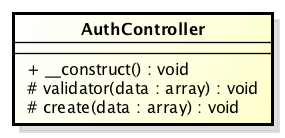
\includegraphics[width=0.5\linewidth]{img/back_end_http_controllers_authController}
\caption[Diagramma della classe AuthController]{Diagramma della classe AuthController}
\label{fig:back_end_http_controllers_authController}
\end{figure}
		\subparagraph{Descrizione}
			AuthController gestisce la registrazione dei nuovi utenti e i loro accessi.
		\subparagraph{Metodi}
			\begin{itemize}
				\item \textbf{+ \_\_construct()}\\
				Il costruttore della classe AuthController.
				\item \textbf{\# validator(data)}\\
				Il metodo si occupa della validazione di tutte le informazioni che riguardano l'utente al momento della registrazione.\\
					\textbf{Argomenti:}
						\begin{itemize}
							\item data : array;
							Array di valori contenente tutti i dati della registrazione di un utente. 
						\end{itemize}
				\item \textbf{\# create(data)}\\
				Il metodo si occupa della creazione di un nuovo utente.\\
					\textbf{Argomenti:}
						\begin{itemize}
							\item data : array;
							Array di valori contenente tutti i dati della registrazione di un utente.
						\end{itemize}
			\end{itemize}
			
	\paragraph{PasswordController}
	\begin{figure}[h]
\centering
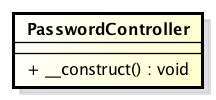
\includegraphics[width=0.5\linewidth]{img/back_end_http_controllers_passwordController}
\caption[Diagramma della classe PasswordController]{Diagramma della classe PasswordController}
\label{fig:back_end_http_controllers_passwordController}
\end{figure}

		\subparagraph{Descrizione}
			PasswordController contiene la logica per aiutare gli utenti per il reset delle loro credenziali di accesso.
		\subparagraph{Metodi}
			\begin{itemize}
				\item \textbf{+ \_\_construct()}\\
				Il costruttore della classe PasswordController.
			\end{itemize}
	